% Name: PID controller
% Description: The error signal split into proportional, integral, and derivative paths and summed.
% Tags: PID, controller, control systems

\usetikzlibrary{arrows.meta, positioning}

\begin{tikzpicture}[
  node distance=5mm and 12mm,
  block/.style={draw, thick, minimum height=11mm, minimum width=24mm},
  sum/.style={draw, thick, circle, inner sep=1pt, minimum size=7mm},
  arrow/.style={-{Stealth}, thick},
]
  \node[block] (i) {$K_i \int_0^t e(\tau)\,d\tau$};
  \node[block, above=of i] (p) {$K_p\, e(t)$};
  \node[block, below=of i] (d) {$K_d\, \dfrac{de}{dt}$};
  \coordinate[left=of i] (split);
  \coordinate[left=10mm of split] (in);
  \node[sum, right=of i] (sum) {$\Sigma$};
  \coordinate[right=10mm of sum] (out);

  \draw[thick] (in) node[left] {$e(t)$} -- (split);
  \fill (split) circle (1.5pt);
  \foreach \b in {p, i, d}
    \draw[arrow] (split) |- (\b);
  \draw[arrow] (p) -| (sum);
  \draw[arrow] (i) -- (sum);
  \draw[arrow] (d) -| (sum);
  \draw[arrow] (sum) -- (out) node[right] {$u(t)$};
\end{tikzpicture}
